
\section{\'Area y longitud de arco}

\subsection{\'Area entre una curva y el eje vertical}


Nostros ya sabemos como encontrar el áre de una regi\'on como la siguiente 
\begin{figure}
 \centering
 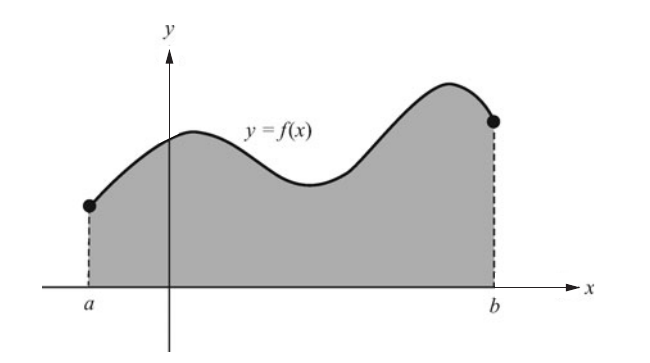
\includegraphics[height=5cm,keepaspectratio=true]{./calculo/fig2901.png}
 % fig2901.png: 0x0 pixel, 300dpi, 0.00x0.00 cm, bb=
 \caption{Área bajo la curva}
 \label{fig:2901}
\end{figure}




El área de la regi\'on acotada por 
$$
x=a, \; x=b, \; y=0, \; y=f(x)
$$
está dada por
$$\displaystyle \int_{a}^{b}f(x) dx$$



Ahora consideremos una regi\'on como la siguiente
\begin{figure}
 \centering
 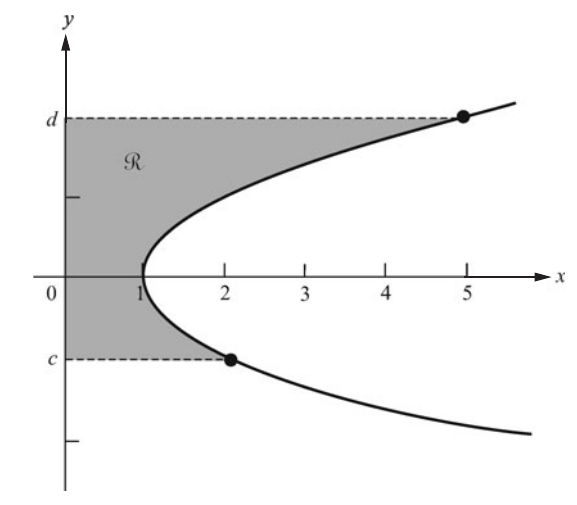
\includegraphics[height=5cm,keepaspectratio=true]{./calculo/fig2902.png}
 % fig2902.png: 0x0 pixel, 300dpi, 0.00x0.00 cm, bb=
 \caption{Área entre curva y eje vertical}
 \label{fig:2902}
\end{figure}




De manera similar, el área de la regi\'on acotada por 
$$
x=0,\; x=g(y),\; y=c,\; y=d
$$ está dada por
$$\displaystyle \int_{c}^{d} g(y)dy$$



\begin{problema}
 \label{exmp:2901}
 Calcule el área de la regi\'on dada en la figura \ref{fig:2903}, que está acotada por el eje $y,$ arriba por $y=2,$ abajo por $y=-1$ y la curva
 $$
 x+y^{2}=4.
 $$ 
 \end{problema}
 


 \begin{figure}
 \centering
 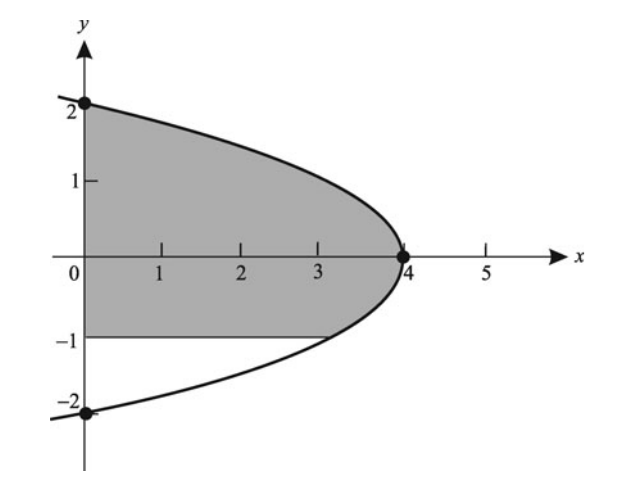
\includegraphics[height=3cm,keepaspectratio=true]{./calculo/fig2903.png}
 % fig2903.png: 0x0 pixel, 300dpi, 0.00x0.00 cm, bb=
 \caption{Área acotada por una parabola}
 \label{fig:2903}
\end{figure}



\subsection{\'Area entre curvas}


Supongamos que $f$ y $g$ son funciones continuas para  \emph{$a \leq x \leq b$}. 



El área $A$ de la regi\'on contenida entre estas dos curvas y los ejes $x=a$ y $x=b$ está dada por la f\'ormula
\[
 \label{29.1}
 A=\int_{a}^{b}\left| f(x)-g(x) \right|dx.
\]




\begin{figure}
 \centering
 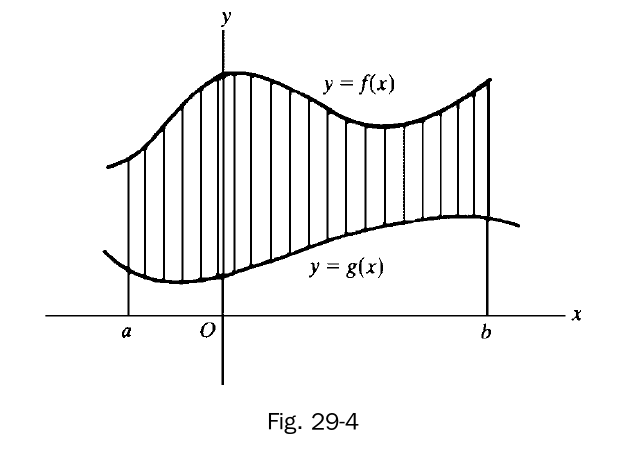
\includegraphics[height=5cm,keepaspectratio=true]{./calculo/fig2904.png}
 % fig2904.png: 0x0 pixel, 300dpi, 0.00x0.00 cm, bb=
 \caption{Área entre curvas (funciones positivas)}
 \label{fig:2904}
\end{figure}



\begin{figure}
 \centering
 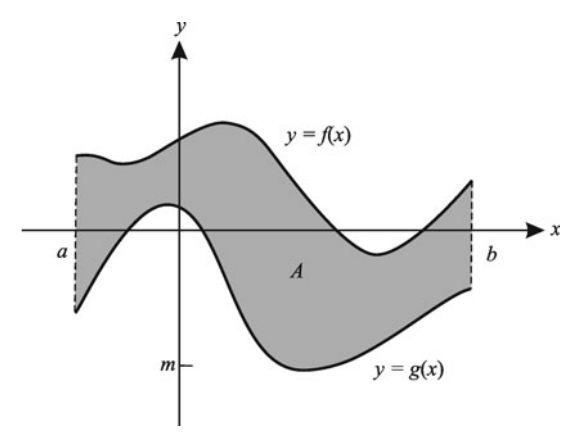
\includegraphics[height=5cm,keepaspectratio=true]{./calculo/fig2905.png}
 % fig2905.png: 0x0 pixel, 300dpi, 0.00x0.00 cm, bb=
 \caption{Área entre curvas}
 \label{fig:2905}
\end{figure}




\begin{figure}
 \centering
 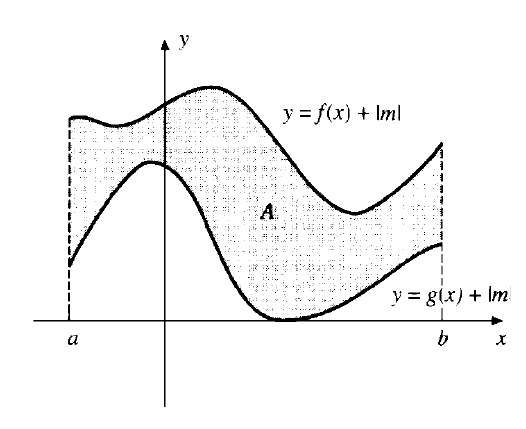
\includegraphics[height=5cm,keepaspectratio=true]{./calculo/fig2906.png}
 % fig2905.png: 0x0 pixel, 300dpi, 0.00x0.00 cm, bb=
 \caption{Deducci\'on de la f\'ormula}
 \label{fig:2906}
\end{figure}




\begin{problema}
 Calcule el área de regi\'on de la figura \ref{fig:2907}, acotada por 
 $$
 x=0,\; x=1,\; y=\dfrac{1}{2}x+2,\; y=x^{2}.
 $$
\end{problema}




\begin{figure}
 \centering
 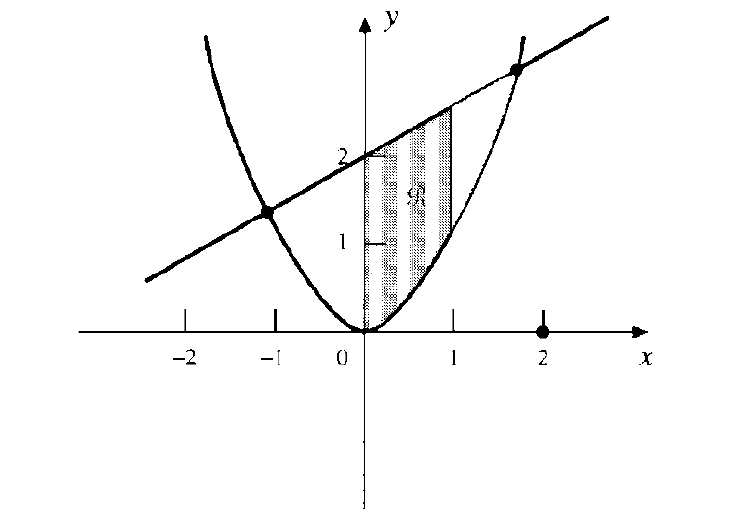
\includegraphics[height=5cm,keepaspectratio=true]{./calculo/fig2907.png}
 % fig2907.png: 0x0 pixel, 300dpi, 0.00x0.00 cm, bb=
 \caption{Área entre línea y parábola}
 \label{fig:2907}
\end{figure}



\subsection{Longitud de arco}


\begin{figure}
 \centering
 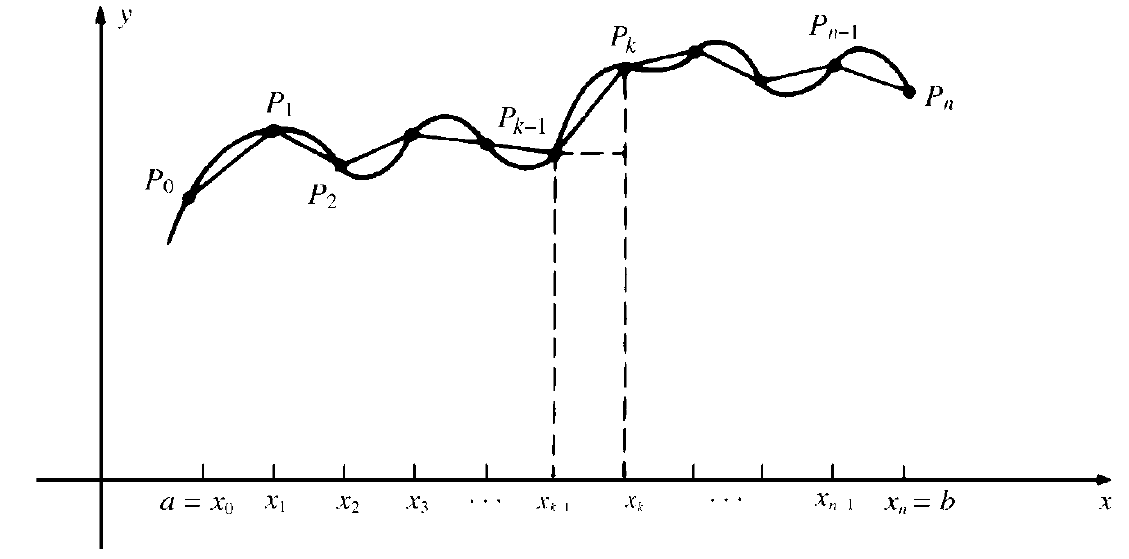
\includegraphics[height=5cm,keepaspectratio=true]{./calculo/fig2908.png}
 % fig2908.png: 0x0 pixel, 300dpi, 0.00x0.00 cm, bb=
 \caption{Aproximación de la longitud de un arco}
 \label{fig:2908}
\end{figure}




Por la f\'ormula de distancia
$$
\overline{P_{k-1}P_{k}}=\sqrt{
\left( x_{k}-x_{k-1} \right)^{2}+
\left( f(x_{k})-f(x_{k-1}) \right)^{2}.
}
$$


Por el teorema del valor medio, existe $x_{k}^{*}\in(x_{k-1},x_{k})$ tal que
$$
f(x_{k})-f(x_{k-1})=\left( x_{k}-x_{k-1} \right)f'(x_{k}^{*})=(\Del x)f'(x_{k}^{*}).
$$

Entonces 
$$
\overline{P_{k-1}P_{k}}=\sqrt{1+\left( f'(x_{k}^{*}) \right)^{2}}(\Del x)
$$



De manera que 
$$
\sum_{k=1}^{n}\overline{P_{k-1}P_{k}}=
\sum_{k=1}^{n}\sqrt{1+\left( f'(x_{k}^{*}) \right)^{2}}(\Del x),
$$ donde $(\Del x)n=b-a.$


Tomando el l\'imite $n \to \infty$ de ambos lados obtenemos que la longitud $L(f,a,b)$ de al arco dado por la curva $f(x)$ en el intervalo $a\leq x \leq b$ esta dado por 
\[
 \label{29.2}
 L(f,a,b)=\int_{a}^{b}\sqrt{1+(f'(x))^{2}}dx.
\]




\begin{problema}
 Encuentre la longitud del arco descrito por la curva $y=x^{3/2}$ de $x=0$ a $x=5.$
\end{problema}



\subsection{Ejemplos}

% Schaum Outline of Calculus

	\begin{problema} %Schaum 29.1
		Encuentre el área acotada por la parábola \[ x=8+y-y^2 , \] el eje $ y $ y las líneas $ y=-1 $ y $ y=3. $
	\end{problema}



	\begin{problema}
		% schaum 29.3
		
		Encuentre el área de la región acotada por las parábolas \[ y= 6x-x^2 \] y \[ y=x^2-2x. \]
	\end{problema}



	\begin{problema}
		%29.7
		Encuentre la longitud de arco de la curva \[ x=3y^{3/2}-1 \] desde $ y=0 $ hasta $ y=4 .$
	\end{problema}



	\begin{problema}
		% 29.9
		Encuentre la longitud de arco de la \emph{catenaria} \[ y=\dfrac{a}{2}\left(e^{x/a} + e^{-x/a}\right) \] desde $ x=0 $ hasta $ x=a $.
	\end{problema}
